% Learned bids over 300 days, one setting at a time (analyze/sweep300_analysis.py).
\begin{figure}[H]
    \centering
    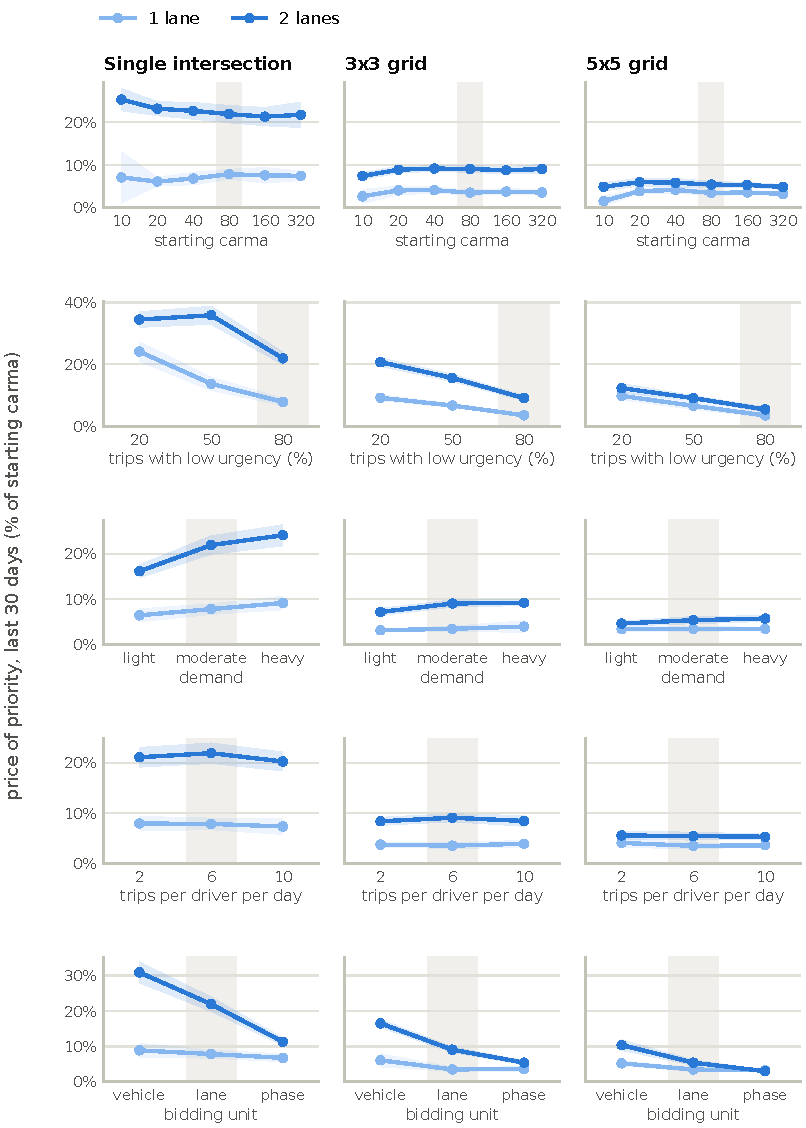
\includegraphics[width=\linewidth]{sweep300_price.pdf}
    \caption{Price of priority after 300 learning days (median contested winning bid as a share of
    starting carma, mean of the last 30 days), changing one setting at a time from the reference
    (shaded: 80 carma, 80\% low-urgency trips, moderate demand, 6 trips per driver, lane bids).
    Mean over the network's auctioned intersections; means of 10 seeds, bands 95\% intervals.
    Bids are whole carma, so with 10 starting carma one unit is 10\%.}
    \label{fig:sweep300_price}
\end{figure}

\begin{figure}[H]
    \centering
    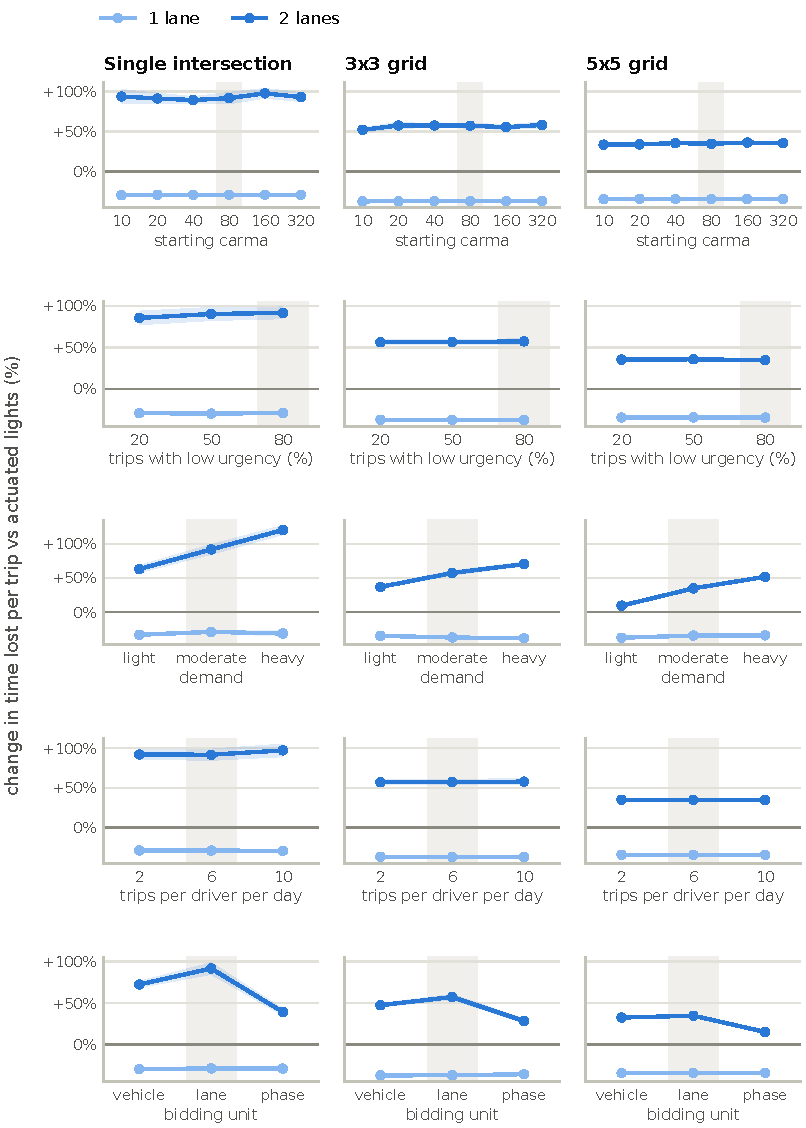
\includegraphics[width=\linewidth]{sweep300_time_lost.pdf}
    \caption{Time lost per trip with learned bids after 300 learning days, compared with actuated
    lights on the same evaluation trips (paired by seed), one setting at a time from the reference
    (shaded). Means of 10 seeds, bands 95\% intervals.}
    \label{fig:sweep300_time_lost}
\end{figure}
